\documentclass[11pt, answers]{exam}

\usepackage{fullpage}
\usepackage{graphicx}
\usepackage{amsmath}
\usepackage{amssymb}
\usepackage{amsthm}
\usepackage{fancyvrb}
\usepackage{amsfonts}
\usepackage{enumerate}
\usepackage{graphicx}
\usepackage{mdframed}
\usepackage{multicol}
\usepackage{verbatim}
\usepackage{tikz}
\usepackage{enumitem}
\usepackage{float}
\usepackage{hyperref}
\usepackage{physics}
\usepackage{bm}
\hypersetup{
    colorlinks=true,
    urlcolor=blue,
}

\parindent0in
\pagestyle{plain}
\thispagestyle{plain}

%% MACRO DEFINITIONS %%

% Names + Dates!
\newcommand{\myname}{Alexander Khosrowshahi}
\newcommand{\assignment}{Homework X}
\newcommand{\duedate}{Month, Day, Year}

\begin{document}

\textbf{Brown University}\hfill\textbf{\myname}\\[0.01in]
\textbf{Course Code -- Course Name}\hfill\textbf{\assignment}\\[0.01in]
\textbf{Prof.\ Professorson}\hfill\textbf{\duedate}\\
\smallskip\hrule\bigskip

\section*{Conceptual Questions}

\begin{questions}

	\question
	The update rule for weights in a single layer, multi-class neural network with cross entropy loss is defined as follows:

	Let $w_{ij}$ be the weight associating the $i$th input feature $x_i$ with the $j$th class. Let $c$ be the index of the correct class for a given input (the {\it label}). The loss and its derivatives are then:

	$$L = -\log(P_c), \ \ \ \ \ \frac{\partial L}{\partial w_{ij}} = \begin{cases}
			(P_j - 1)x_i & j = c    \\
			P_j x_i      & j \neq c
		\end{cases}$$
	We use these partials with a learning rate $\alpha$ to descend along the gradient:
	$$w_{ij} = w_{ij} - \frac{\partial L}{\partial w_{ij}}\alpha$$

	Derive the above rules from the original definition of cross-entropy loss.

	\begin{quote}
		{\bf Hint:} Consider both cases of $j$, and start by expanding out $L$.
	\end{quote}

	\question
	In classification problems, we assign a likelihood probability to each class and use a loss function that outputs a loss based on this probability. Can you use MSE loss for classification tasks? Why or why not? Why is cross-entropy loss most commonly used for classification? (3-5 sentences)

	\begin{quote}
		{\bf Hint:} Think about how each loss function is shaped, the inputs that they take in, and the range of each function's inputs.
	\end{quote}

	\newpage % just for from-scratch aesthetics. Feel free to remove

	\question
	In lecture, you learned about gradient descent. What is a gradient? How is it different from a partial derivative? How do they relate? ({\it 2-4 sentences})

	\question
	Consider the formula for updating our weights:
	$$\Delta w = -\alpha \frac{\partial L}{\partial w}$$
	Why do we negate this quantity? What purpose does this serve? ({\it 2-4 sentences})

	\question
	During gradient descent, we calculate the partial derivative of loss ($L$) with respect to each weight $(w_{ij})$. Why must we do this for every weight? Why can't we do this for some weights? ({\it 1-3 sentences})

	\question
	In practice, most operations during gradient descent are vectorized. Why do we do this? Why might this make it beneficial to train the model on a GPU? ({\it 1-2 sentences})

	\question
	Consider the following plot of a loss function for some neural network:
	\begin{figure}[H]
		\caption{Loss Manifold Visualization}
		\centering
		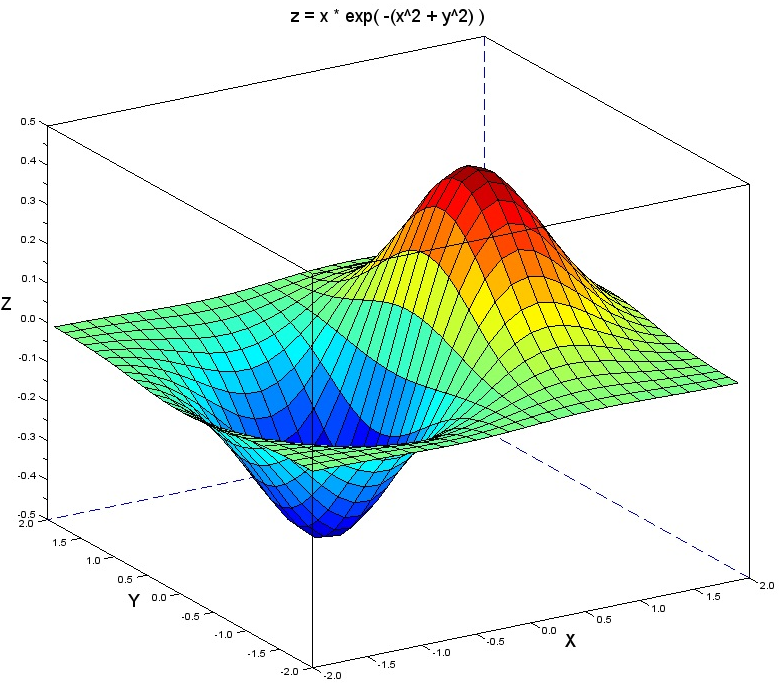
\includegraphics[width=0.7\linewidth]{../images/hw2-loss.png}
		\label{fig:label}
	\end{figure}
	Where should gradient descent end up on the graph? How many weights does this model have? If our model starts training at $(-2, 2, 0)$, will the loss function ever reach the absolute minimum? Why? Assume the loss function at this point is {\it perfectly flat}. ({\it 3-5 sentences})

\end{questions}

\newpage % just for from-scratch aesthetics. Feel free to remove

\section{Bonus Questions}

\begin{figure}[H]
	\caption{Sample Neural Network}
	\centering
	\includegraphics[width=0.7\linewidth]{../images/bonus-model.png}
	\label{fig:label}
\end{figure}

For the following questions, the answers will have to do with the following four functions: \textit{get$\_$input$\_$gradients()}, \textit{get$\_$weight$\_$gradients()}, \textit{compose$\_$input$\_$gradients()}, and \textit{compose$\_$weight$\_$gradients()}. Note that through the Diffable class, each of the layers shown above ($f\_1$, $f\_2$, $L$)  either individually  implement or inherit these functions.

\begin{questions}
	\question
	To initialize backpropagation, which function must you call on which layer? What partial derivative(s) would this return? (Hint: Think back to HW1)

	\question
	At layer $f_1$, what shape are the partials that `get$\_$input$\_$gradients(J)` and `get$\_$weight$\_$gradients(J) `return? Imagine that x is a vector of length $m$ and that $w_1$ is a weight matrix of size $(m, r)$. `J` will be the correct upstream gradient. (Hint: Think back to HW1)

	\question
	At layer $f_1$, what shape are the partials that `compose$\_$input$\_$gradients(J)` and `compose$\_$weight$\_$gradients(J)` return? For this to occur, how must each function resolve the input dimension? What upstream partial is necessary for these functions?

	\question
	At layer $f_1$, how does `compose$\_$input$\_$gradients(J)`,  resolve the input dimension difference? More specifically, how does this function create a gradient the same shape as the inputs to this layer $(N,m)$? Be sure to reference the matrix multiplication at line 200 in `core.py`. Imagine that $w_2$ is a weight matrix of size $(r,1)$.

\end{questions}

\section*{More Bonus (More math)}

\begin{questions}
	\question
	In your introductory calculus class, you were likely exposed to the following simple algorithm for finding the minimum of a function: take the derivative of the function, set it to zero, then solve the equation.

	Neural networks are differentiable, so why don't we use this algorithm (instead of gradient descent) to minimize the loss? ({\it 1-4 sentences})

	\question
	Prove that SGD with batch size of 1 gives an {\it unbiased estimate} of the "true gradient" (the gradient calculated over the entire training set). Assume that the batch is selected uniform-randomly from the full training set.

	\begin{quote}
		{\bf Hints:}
		\begin{enumerate}
			\item Recall that an estimator $\hat{f}$ is an unbiased estimator of a function $f$ if $\mathbb {E}[\hat f] = f$.

			\item Both expectation and differentiation are linear operators.
		\end{enumerate}
	\end{quote}

	In the assignment, you will see that even a single-layer neural network can classify the digit with pretty good accuracy. Still, there are several ways in which one could improve the accuracy of the model. The paper in the link below suggests and easy way to increase the performance without changing the architecture of our network: training several identical models! Please read the following paper (found here) and answer the following questions:

	\question
	What is the committee? Why would it help increase the performance of the model?

	\question
	What is the preprocessing they implement in this paper? How does this preprocessing prevent the models' errors from being strongly correlated?

\end{questions}

\end{document}
